% ==========================================
%  Category macros
% ==========================================
\newcommand{\cat}[1]{\mathbf{#1}}
\newcommand{\OGraph}{\cat{OGraph}}
\newcommand{\Graph}{\cat{Graph}}
\newcommand{\Hyp}{\cat{Hyp}}
\newcommand{\Set}{\cat{Set}}

% ==========================================
%  AION / RMG Names
% ==========================================
\newcommand{\RMG}{\mathrm{RMG}}
\newcommand{\Hist}{\mathrm{Hist}}

% Inline project names (math-safe)
\newcommand{\AION}{\text{AI}\textOmega\text{N}}
\newcommand{\COMPUTER}{\text{C}\textOmega\text{MPUTER}}
\newcommand{\AIONWordmarkSerif}{\textrm{AION}}
\newcommand{\AIONInline}{\textrm{AION}}
\newcommand{\AIONSignature}[1][1]{\AIONWordmarkSerif}
\newcommand{\AIONProjectURL}{\url{https://flyingrobots.dev}}
\newcommand{\FULL}{\textbf{FULL}}
\newcommand{\ZK}{\textbf{ZK}}
\newcommand{\OPAQUE}{\textbf{OPAQUE}}

% ==========================================
%  Rewrite / Footprint helpers
% ==========================================
% We use \rightsquigarrow to denote rewrite steps.
\newcommand{\Rewrite}{\rightsquigarrow}
\newcommand{\To}{\rightarrow}
\newcommand{\mono}{\hookrightarrow}

\newcommand{\Del}{\mathrm{Del}}
\newcommand{\Use}{\mathrm{Use}}
\newcommand{\Foot}{\mathrm{Foot}}
\newcommand{\RMGState}{\mathrm{RMGState}}
\newcommand{\Recon}{\mathrm{Recon}}
\newcommand{\Apply}{\mathrm{Apply}}
\newcommand{\Trans}{\mathrm{Trans}}

% ==========================================
%  Theorem environments
% ==========================================
\theoremstyle{plain}
\newtheorem{theorem}{Theorem}[section]
\newtheorem{lemma}[theorem]{Lemma}
\newtheorem{proposition}[theorem]{Proposition}
\newtheorem{corollary}[theorem]{Corollary}

\theoremstyle{definition}
\newtheorem{definition}[theorem]{Definition}
\newtheorem{example}[theorem]{Example}
\newtheorem{remark}[theorem]{Remark}

% ==========================================
% ==========================================
%  Wordmark: Display + Inline (uses serif roman + Greek Omega)
% ==========================================
\renewcommand{\AIONWordmarkSerif}{%
  {\rmfamily\Large A\kern0.15em I\kern0.2em \ensuremath{\Omega}\kern0.1em N}%
}

\renewcommand{\AIONInline}{%
  {\rmfamily A\kern0.12em I\kern0.16em \ensuremath{\Omega}\kern0.1em N}%
}

% ---------------------------------------------------------
% AION LOGO (circle + diamond + square)
% Numeric values tuned for the current wordmark size; see comments below.
% ---------------------------------------------------------
\pgfkeys{/aionlogo/.cd,
  scale/.store in=\aionlogoScale, scale=1,
  radius/.store in=\aionlogoRadius, radius=1.05,
  square/.store in=\aionlogoSquare, square=0.55,
  outerwidth/.store in=\aionlogoOuterWidth, outerwidth=0.52pt,
  innerwidth/.store in=\aionlogoInnerWidth, innerwidth=0.32pt
}

\newcommand{\AIONLogo}[1][1]{%
  \pgfkeys{/aionlogo,scale=#1}%
  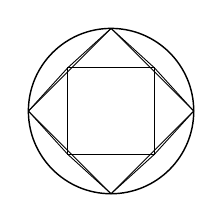
\begin{tikzpicture}[
      scale=\aionlogoScale,
      baseline=-0.55ex,% aligns with the wordmark baseline
      line cap=round,
      line join=round]
    \pgfmathsetmacro{\R}{\aionlogoRadius}
    \pgfmathsetmacro{\s}{\aionlogoSquare}
    \path (0,\R) coordinate (N)
          (0,-\R) coordinate (S)
          (\R,0) coordinate (E)
          (-\R,0) coordinate (W)
          (\s,\s) coordinate (NE)
          (-\s,\s) coordinate (NW)
          (\s,-\s) coordinate (SE)
          (-\s,-\s) coordinate (SW);

    \draw[line width=\aionlogoOuterWidth] (0,0) circle (\R);
    \draw[line width=\aionlogoInnerWidth] (N) -- (E) -- (S) -- (W) -- cycle;
    \draw[line width=\aionlogoInnerWidth] (NW) rectangle (SE);
    \draw[line width=\aionlogoInnerWidth] (N) -- (NE);
    \draw[line width=\aionlogoInnerWidth] (N) -- (NW);
    \draw[line width=\aionlogoInnerWidth] (S) -- (SE);
    \draw[line width=\aionlogoInnerWidth] (S) -- (SW);
    \draw[line width=\aionlogoInnerWidth] (E) -- (NE);
    \draw[line width=\aionlogoInnerWidth] (E) -- (SE);
    \draw[line width=\aionlogoInnerWidth] (W) -- (NW);
    \draw[line width=\aionlogoInnerWidth] (W) -- (SW);
    % Node dots intentionally omitted to keep the emblem minimal.
  \end{tikzpicture}%
}

\renewcommand{\AIONSignature}[1][0.28]{%
  % Raise/kerning values tuned for optical alignment with the wordmark.
  \raisebox{0.02em}{\smash{\AIONLogo[#1]}}\kern0.65em{\AIONWordmarkSerif}%
}
